\documentclass[11pt,twoside]{book}

\usepackage[utf8]{inputenc}
\usepackage[english]{babel}

\usepackage{geometry}
\geometry{papersize={145mm,200mm}} % 60x84/16 is 145 mm x 200 mm
\geometry{tmargin=1.6cm,bmargin=1.6cm,lmargin=2cm,rmargin=2cm}

\usepackage{tikz}
\usetikzlibrary{arrows,arrows.meta}

\begin{document}

\pagestyle{empty}

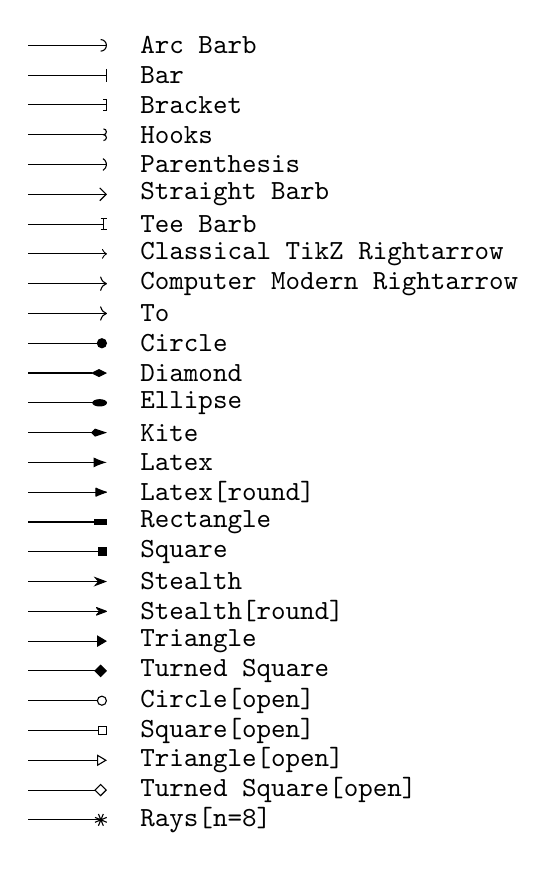
\begin{tikzpicture}[yscale=-1, y=2.5ex]
	\foreach \tip [count=\i] in {
		Arc Barb, Bar, Bracket, Hooks, Parenthesis, Straight Barb, Tee Barb,
		Classical TikZ Rightarrow, Computer Modern Rightarrow, To,
		Circle, Diamond, Ellipse, Kite, Latex, Latex[round], Rectangle, Square, Stealth, Stealth[round], Triangle, Turned Square,
		Circle[open], Square[open], Triangle[open], Turned Square[open],
		Rays[n=8]
  } {
	\draw [-{\tip}] (0, \i) to ++(1, 0) node [right] {\hspace{3mm}\texttt{\tip}};
  }
\end{tikzpicture}

\end{document}
